\subsection{Setup}


Considering the setup shown in Figure \ref{fig:sensor_traj}. A sensor moves at a constant speed $v$ at a fixed altitude $d$ above an infinitely long straight cable carrying a DC current $I$. The system is described in a CPA frame of reference, whose origin is located at the closest point of approach (CPA) and which is rotated by an angle $\psi$ relative to the magnetic north. The sensor crosses the cable at an angle $\theta$.

\begin{figure}[h]
\centering
\begin{minipage}{0.48\linewidth}
    \centering
    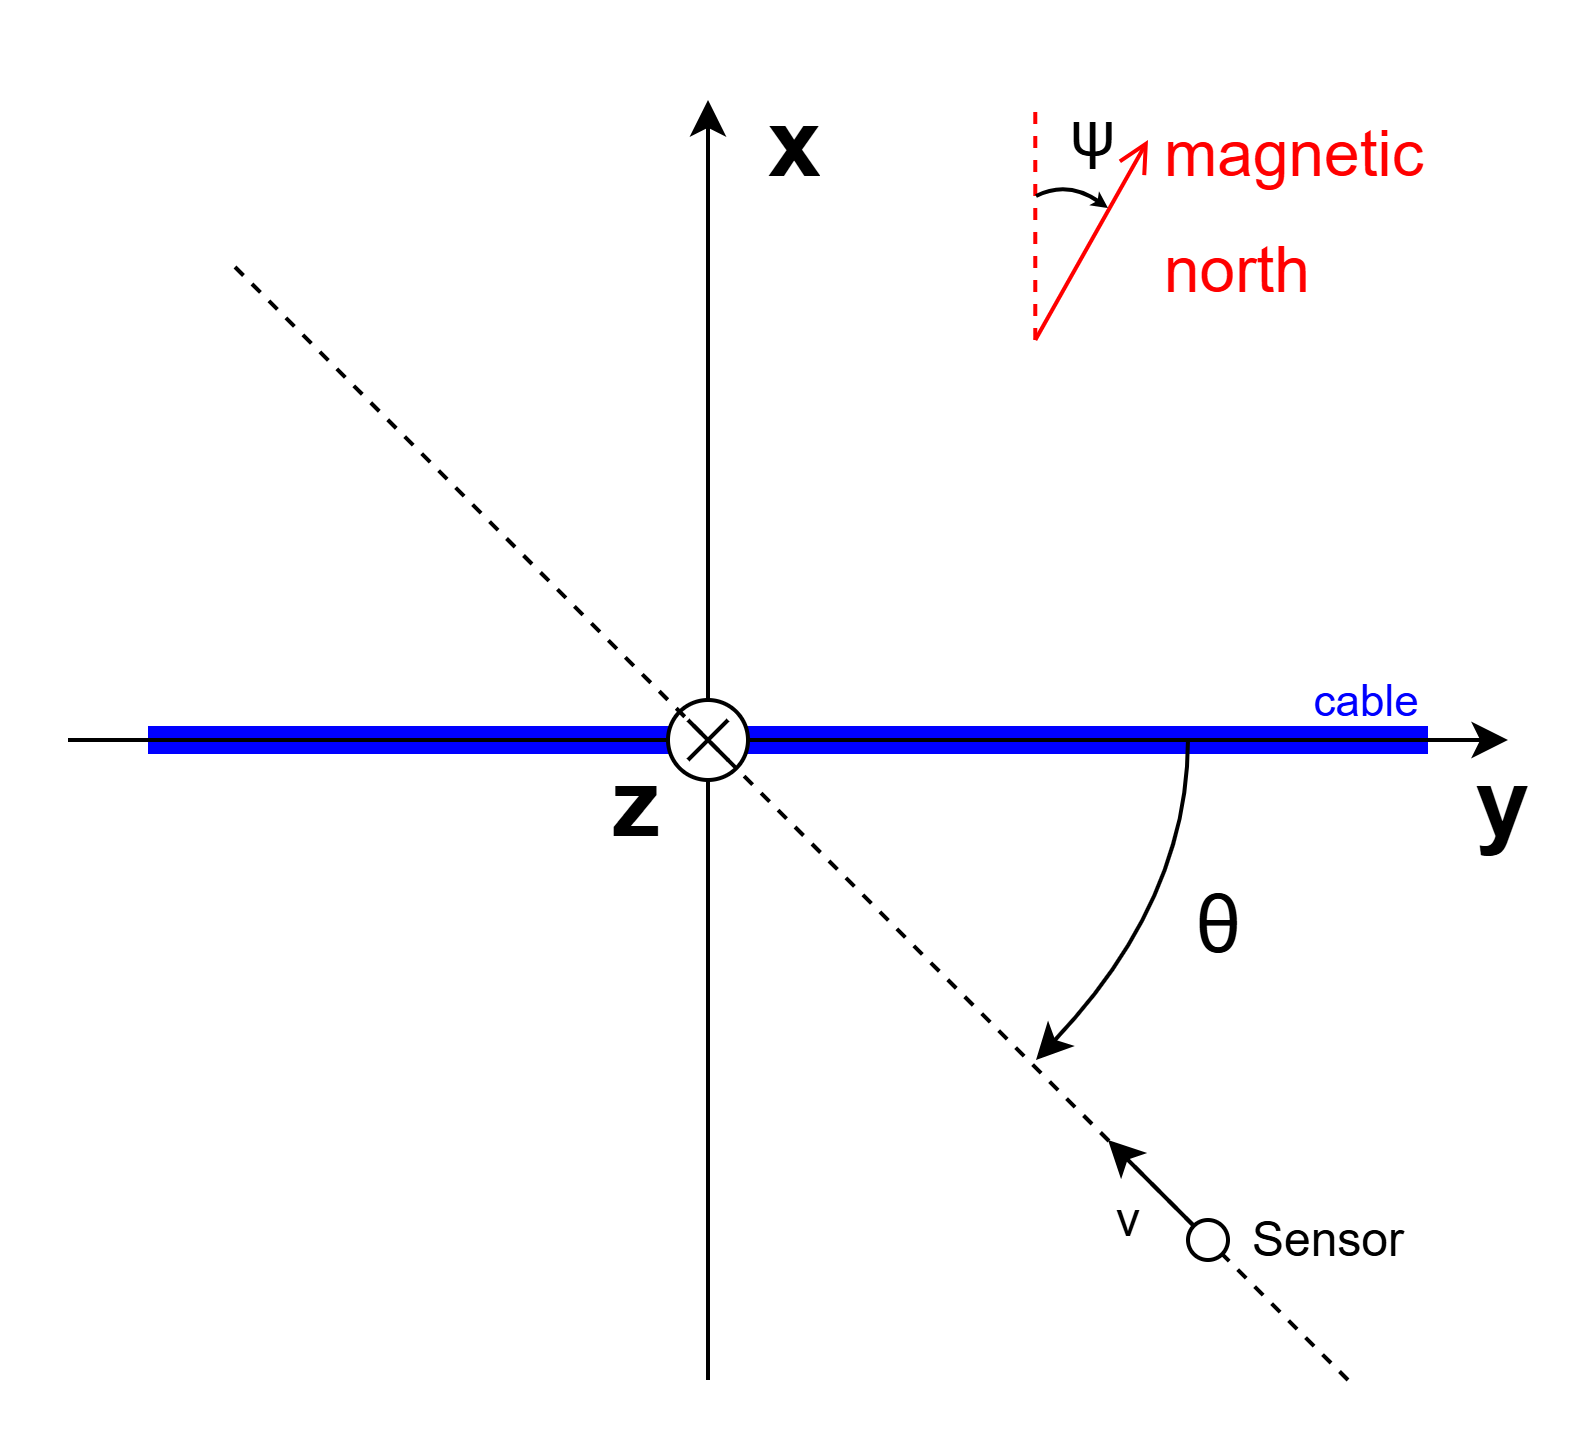
\includegraphics[width=\linewidth]{methodology/figures/sensor_trajectory1.png}
\end{minipage}
\hfill
\begin{minipage}{0.48\linewidth}
    \centering
    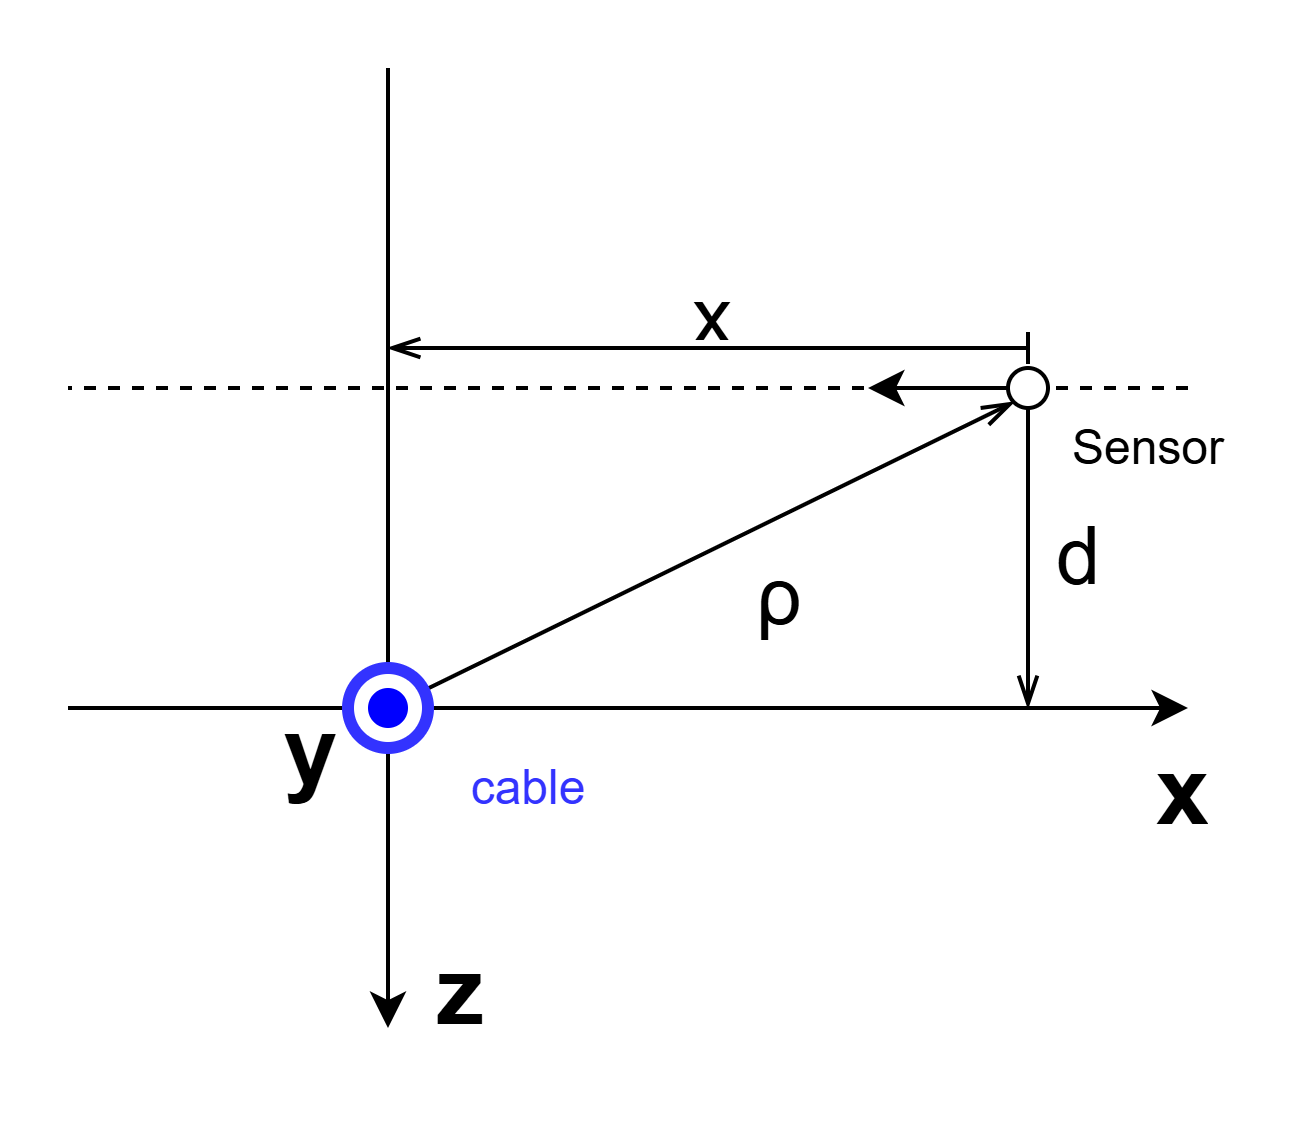
\includegraphics[width=\linewidth]{methodology/figures/sensor_trajectory2.png}
\end{minipage}
    \caption{Sensor trajectory in the CPA frame of reference, on the left (top down view), on the right (profile view)}
    \label{fig:sensor_traj}
\end{figure}

\highlight{Starting from the expression of the magnetic field in the CPA frame of reference, and noting that, as an underwater telecommunications cable, the return current is via the seawater, which motivates modeling the cable as an infinite straight conductor carrying current in a single direction, under this assumption, the magnetic field is obtained using the classical Biot–Savart law:}

\begin{equation*}
    \vec{B} = \frac{\mu_0}{4\pi} \int \frac{I \, d\vec{\ell} \times \hat{r}}{r^2}
\end{equation*}

where, in our application, \(d\vec{\ell}\) is \(d\vec{y}\), and \(\vec{r}\) is \(\vec{\rho}\)   (the radial sensor position relative to the cable), further development will give :
\highlight{
\begin{equation}
    \vec{B} = \frac{\mu_0 I}{2\pi \rho}\,\vec{e}_{az}
    \label{eq:mag_field}
\end{equation}

where $\vec{e}_{az}$ is the azimuthal unit vector (right-hand rule).

\begin{equation*}
\vec{e}_{az} = \frac{d\vec{y} \times \vec{\rho}}{\rho}
= \frac{1}{\rho}
\begin{pmatrix}
0 \\ 1 \\ 0
\end{pmatrix}
\times
\begin{pmatrix}
-x \\ 0 \\ d
\end{pmatrix}
=  \frac{1}{\rho}
\begin{pmatrix}
d \\ 0 \\ x
\end{pmatrix}
\end{equation*}
}
Although \(\vec{B}\) is inherently a spatial field, the sensor motion causes it to be observed as a time-varying signal \(\vec{B}_s(t) = \vec{B}(\mathbf{\rho}(t))\).

Assuming a rectilinear trajectory, the sensor position along the \(x\)-axis is given by
\(
x(t) = v t \sin(\theta)
\)
and $\rho(t) = \sqrt{x^2(t) + d^2}$.

For simplicity, we assume that the sensor does not rotate, \textit{i.e., its local \(x\) and \(z\) axes remain aligned with those of the CPA frame at all times}.

The measured magnetic field in the sensor frame is then
\begin{equation*}
    \vec{B}_s(t) =  \frac{\mu_0 I}{2 \pi} 
    \begin{pmatrix}
        \dfrac{d}{\rho^2(t)} \\[6pt]
        0 \\[6pt]
        \dfrac{x(t)}{\rho^2(t)}
    \end{pmatrix},
\end{equation*}

This expression can be normalized with respect to time, velocity, and trajectory angle \(\theta\) by introducing the dimensionless variable
\[
\tau = \frac{x(t)}{d} = \frac{v t \sin(\theta)}{d}.
\]

After simple factorization, the normalized magnetic field measurement becomes
\begin{equation*}
    \vec{B}_s(\tau) = \frac{\mu_0 I}{2 \pi d}
    \begin{pmatrix}
        \dfrac{1}{1+\tau^2} \\[6pt]
        0 \\[6pt]
        \dfrac{\tau}{1+\tau^2}
    \end{pmatrix}.
\end{equation*}